\documentclass[tikz,border=8pt]{standalone}
% Shared look for every TikZ diagram. Load with \input{../../tools/tikz-style.tex}
\usepackage[T1]{fontenc}
\usepackage{lmodern}
\renewcommand{\sfdefault}{lmr}  % diagrams use the same serif as the text
\usetikzlibrary{arrows.meta, positioning, shapes.geometric, calc, fit, backgrounds}
\definecolor{cblue}{HTML}{4C78A8}
\definecolor{corange}{HTML}{F58518}
\definecolor{cgreen}{HTML}{54A24B}
\definecolor{cred}{HTML}{E45756}
\definecolor{cpurple}{HTML}{B279A2}
\definecolor{cgrey}{HTML}{6B6B6B}
\tikzset{
  every picture/.style={font=\sffamily, line width=1.2pt},
  box/.style={draw=#1, fill=#1!12, rounded corners=4pt, align=center, inner sep=7pt, minimum height=1.1cm},
  box/.default=cgrey,
  arrow/.style={-{Stealth[length=3mm]}, draw=cgrey, line width=1.4pt},
  title/.style={font=\sffamily\bfseries\Large},
  note/.style={font=\sffamily\small, text=cgrey, align=center},
}
\AtBeginDocument{\hyphenpenalty=10000 \exhyphenpenalty=10000}

\begin{document}
% Section 5: the whole sentence at once for "money bank grows" (3 words, 50 numbers each):
% S = X X^T (3 x 3), W = row-wise softmax of S, Y = W X (3 x 50).
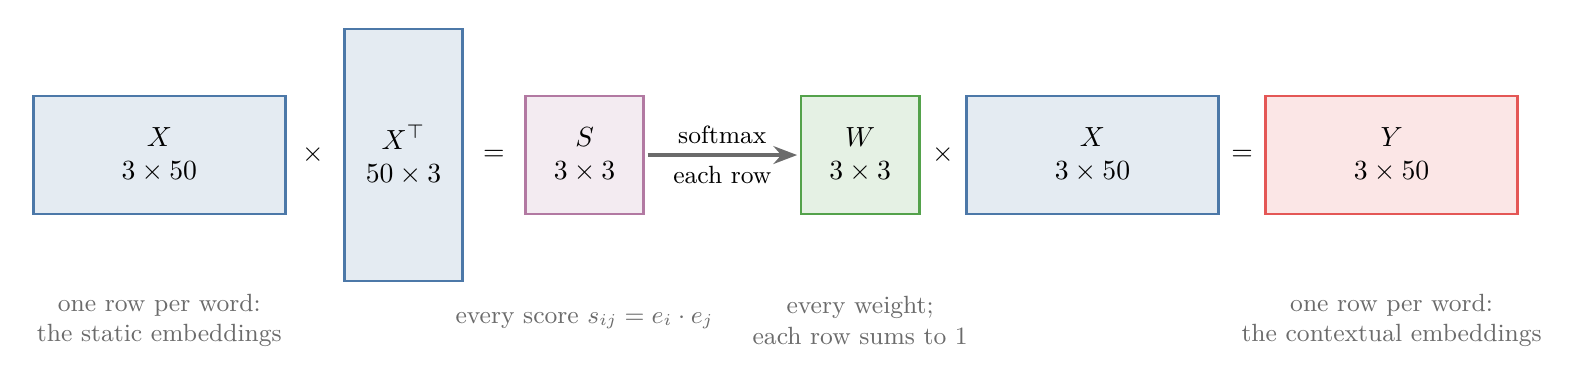
\begin{tikzpicture}[m/.style={draw=#1, fill=#1!15, line width=1pt, font=\sffamily, align=center}]
  \node[m=cblue, minimum width=3.2cm, minimum height=1.5cm] (X) at (0, 0) {$X$\\$3 \times 50$};
  \node at (1.95, 0) {$\times$};
  \node[m=cblue, minimum width=1.5cm, minimum height=3.2cm] (XT) at (3.1, 0) {$X^{\top}$\\$50 \times 3$};
  \node at (4.25, 0) {$=$};
  \node[m=cpurple, minimum width=1.5cm, minimum height=1.5cm] (S) at (5.4, 0) {$S$\\$3 \times 3$};
  \draw[arrow] (6.2, 0) -- node[above, font=\sffamily\small] {softmax} node[below, font=\sffamily\small] {each row} (8.1, 0);
  \node[m=cgreen, minimum width=1.5cm, minimum height=1.5cm] (W) at (8.9, 0) {$W$\\$3 \times 3$};
  \node at (9.95, 0) {$\times$};
  \node[m=cblue, minimum width=3.2cm, minimum height=1.5cm] (X2) at (11.85, 0) {$X$\\$3 \times 50$};
  \node at (13.75, 0) {$=$};
  \node[m=cred, minimum width=3.2cm, minimum height=1.5cm] (Y) at (15.65, 0) {$Y$\\$3 \times 50$};
  \node[note] at (0, -2.1) {one row per word:\\the static embeddings};
  \node[note] at (5.4, -2.1) {every score $s_{ij} = e_i \cdot e_j$};
  \node[note] at (8.9, -2.1) {every weight;\\each row sums to 1};
  \node[note] at (15.65, -2.1) {one row per word:\\the contextual embeddings};
\end{tikzpicture}
\end{document}
